\section{Evaluation}
\begin{frame}
    \frametitle{Evaluation - Vorgehen}
    \begin{itemize}
        \item 20 von Hand annotierte Punktwolken aus \acs{d435}
            \pnote{Verschiedene Szenarien, zur hälfte mit Rampe}
            \pause
        \item Insgesamt 47 Objekte (22 Hindernisse/Fußgänger, 25 Schilder)
            \pause
        \item \acf{iou} von Bounding Boxes
            \pnote{Zwischen Referenzdaten und Messung}
    \end{itemize}
\end{frame}

\begin{frame}
    \frametitle{Evaluation - Verbesserungen}
    \begin{table}
        \centering
        \begin{tabular}{c|c|ccc}
            \toprule
            Algorithmus & Detektionsrate & Pr & Rc & $F_1$ \\
            \midrule
            \cite{AttBen17} Lidar &                     & \onslide<3->{86\%} & \onslide<4->{83\%} & \onslide<5->{85\%} \\
            \cite{AttBen17} Stereo & \onslide<2->{79\%} & \onslide<3->{86\%} & \onslide<4->{90\%} & \onslide<5->{86\%} \\
            Vorgeschlagen &          \onslide<2->{81\%} & \onslide<3->{89\%} & \onslide<4->{92\%} & \onslide<5->{90\%} \\
            \bottomrule
        \end{tabular}
    \end{table}
\end{frame}

\begin{frame}
    \frametitle{Vergleich aktuelle Hindernisserkennung}
    Vergleich nur auf Basis von Hindernissen
    \begin{table}
        \centering
        \begin{tabular}{c|cc}
            \toprule
            Algorithmus & \multicolumn{2}{c}{Durchschnittliche 2D-IoU} \\
             & Detektionen & Alle Objekte\\
            \midrule
            Hindernisserkennung & \onslide<2->{0.48} & \onslide<3->{0.087} \\
            Vorgeschlagen       & \onslide<2->{0.44} & \onslide<3->{0.38} \\
            \bottomrule
        \end{tabular}
    \end{table}
\end{frame}

\begin{frame}
    \frametitle{Analyse der Rechenzeit}
    Daten von Referenzsystem vergleichbar mit Fahrzeug
    \begin{table}
        \begin{tabular}{l|S[table-format=2.2]S[table-format=1.3]}
            \toprule
             & {Mittelwert} & {Standardabweichung} \\
            \midrule
            Segmentierung & 2.1ms & 0.49ms \\
            Clustering & 1.2ms & 0.52ms \\
            Extraktion  & 0.62ms & 0.25ms \\
            Klassifikation & 15ms & 10ms \\
            Bounding Box & 0.73ms & 0.29ms \\
            Bodenschätzung & 0.12ms & 0.046ms \\
            \midrule
            Gesamt & 19ms & 11ms \\
            \bottomrule
        \end{tabular}
    \end{table}
\end{frame}

\begin{frame}
    \frametitle{Echtweltdaten - Kitti}
    \begin{columns}
        \begin{column}{.4\textwidth}
            \begin{itemize}
                \item Stereo-berechnung mit Semi-Global Block Matching
                \item<2-> Kleiner Kameraabstand ($\si{0,54\m}$)
                \item<3-> Punktwolke ungenau
                \item<4-> Detektion bis ca. $\si{10\m}$ möglich
            \end{itemize}
        \end{column}
        \begin{column}{.6\textwidth}
            \begin{figure}[h!]
                \centering
                \begin{tikzpicture}
                    \node[anchor=south west,inner sep=0] at (0,0) {
                        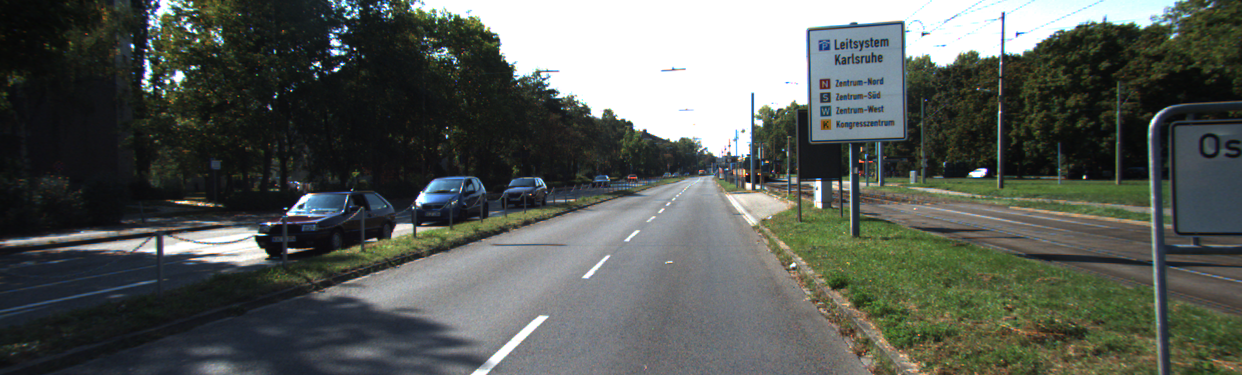
\includegraphics[width=\textwidth,trim={6cm 2cm 22cm 5cm},clip]{../Material/kittiBadImage.png}
                    };
                    \draw[red,ultra thick,rounded corners] (1.1,0.8) rectangle (3,1.8);
                    \draw[green,ultra thick,rounded corners] (3.1,1.2) rectangle (4.2,1.9);
                \end{tikzpicture}
            \end{figure}

            \begin{figure}[h!]
                \centering
                \begin{tikzpicture}
                    \node[anchor=south west,inner sep=0] at (0,0) {
                        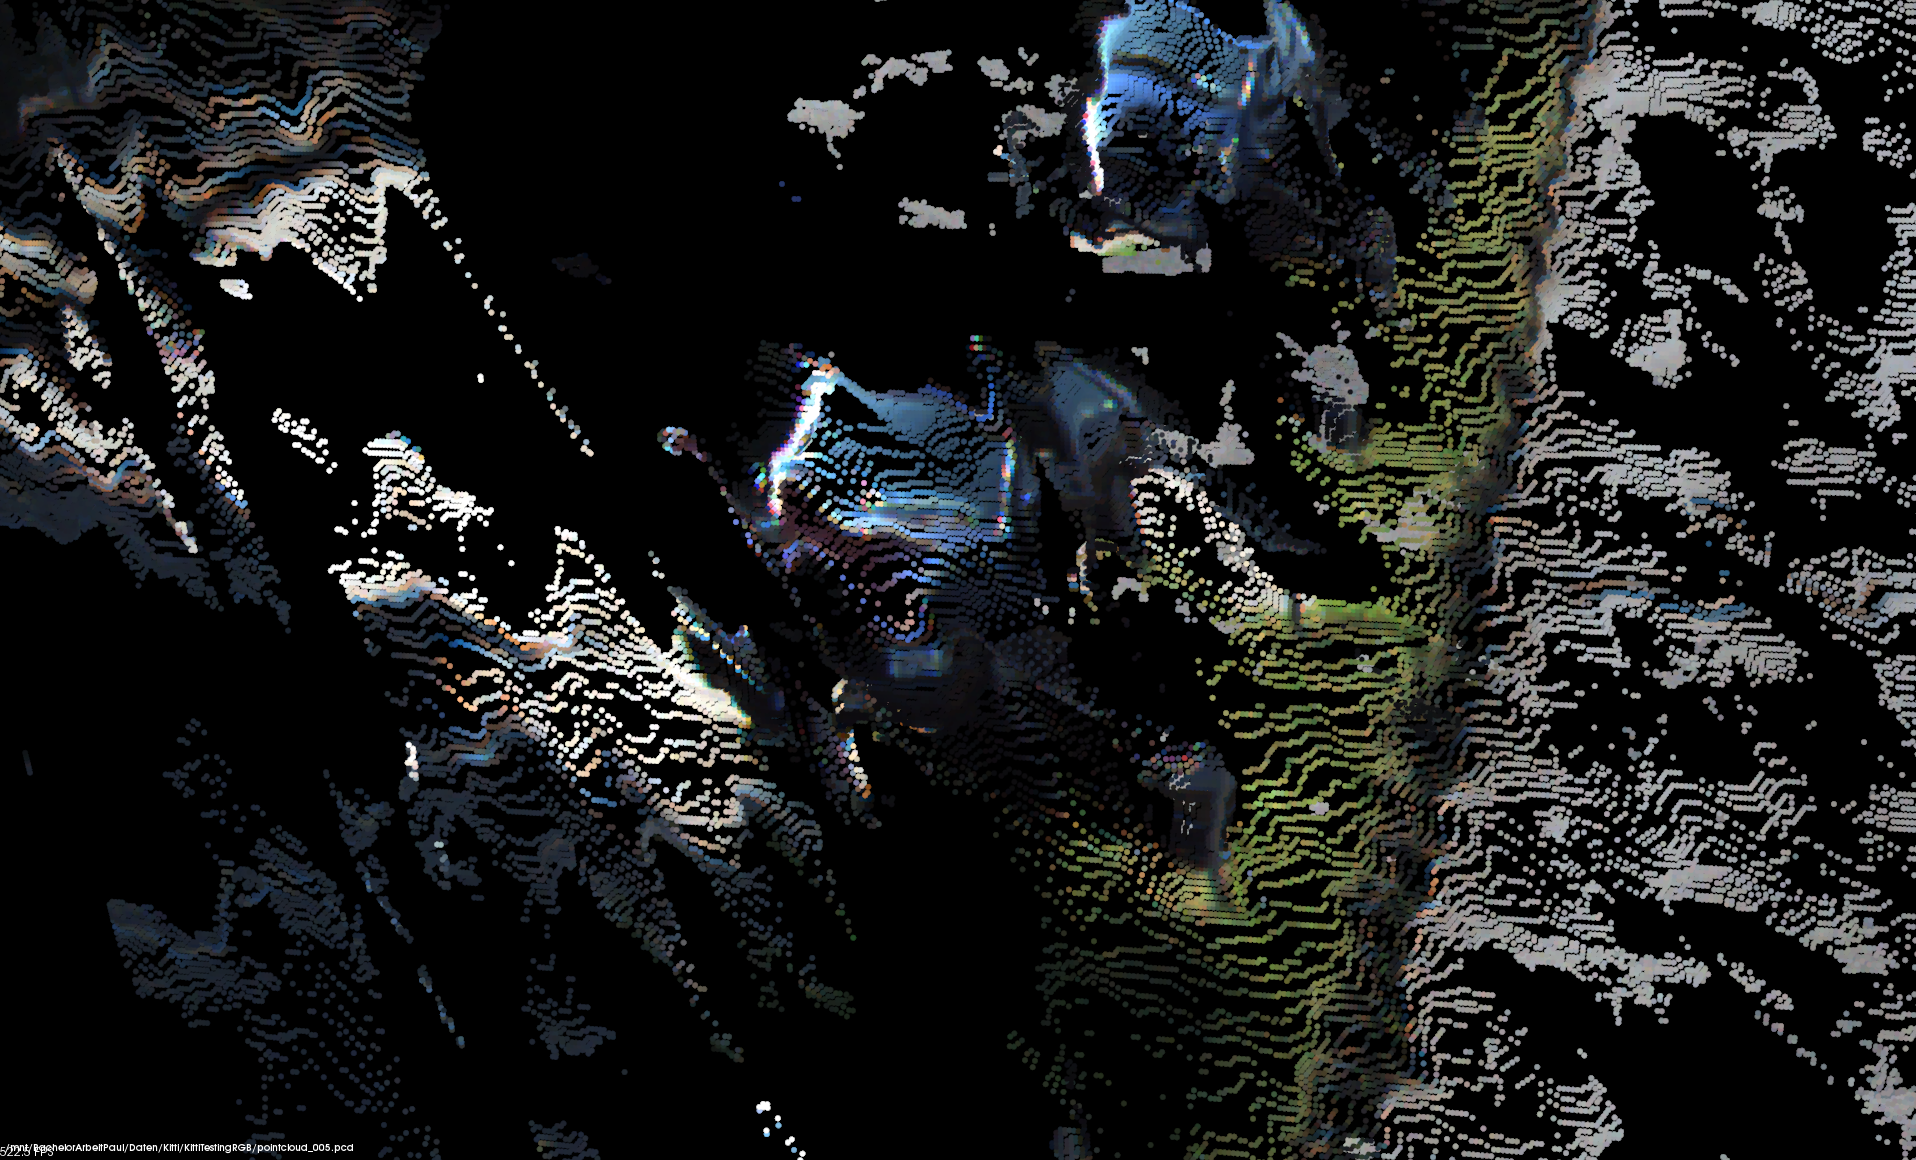
\includegraphics[width=\textwidth]{../Material/kittiBad.png}
                    };
                    \draw[red,ultra thick,rounded corners] (2.1,1.4) rectangle (3.6,2.5);
                    \draw[green,ultra thick,rounded corners] (3.2,2.8) rectangle (4.1,3.5);
                \end{tikzpicture}
            \end{figure}
        \end{column}
    \end{columns}
\end{frame}

\begin{frame}
    \frametitle{Echtweltdaten - Lehr}
    \begin{itemize}
        \item Bessere Punktwolke
            \pause
        \item Einfaches Szenario
            \pause
        \item Ermöglicht Detektion bis ca. $\si{50\m}$
            \pause
        \item Detektionsrate: 88\%
            \pnote{für Carolo: 81\%}
            \pause
        \item Durchschnittliche \ac{iou}: 0.53 (2D), 0.43 (3D)
            \pnote{für Carolo, 0.44, 0.33}
    \end{itemize}
\end{frame}
